%\documentclass[12pt]{article}
%\usepackage[a4paper, margin=1in]{geometry} 
%\usepackage{graphicx} 
%\usepackage{hyperref}
%\usepackage{float}
%\usepackage{multicol}
%\usepackage{amsmath}
%\usepackage[font=small, labelfont=bf]{caption}
%
%\begin{document}

%
% Sequence distance
%
\subsection{Sequence distance}
Distances can be also used to indicate the similarity of an alignment.

%
% Edit distance
%
\subsubsection*{Edit distance}
The Levenshtein distance is one of the most commonly used edit distances in computer science.
\begin{align*}
\mathrm{Insertion}: & \quad AC  \rightarrow AGC  & (\varepsilon  \rightarrow G) \\
\mathrm{Deletion}: & \quad ATC \rightarrow AC & (T \rightarrow \varepsilon) \\
\mathrm{Substitution}: & \quad AAA \rightarrow ATA &  (A \rightarrow T) 
\end{align*}

%
% Scoring scheme for Levenshtein distance
%
\subsubsection*{Scoring scheme for Levenshtein distance}
\begin{itemize}
\item $R_{ab}$ = 0 for a = b
\item $R_{ab}$ = -1 for a $\neq$ b
\item g = 1
\end{itemize}

%
% Distance from DP score
%
\subsubsection*{Distance from DP score}
Given the best score $T$ from DP, the edit distance $d$ is $-T$.
\bigskip  

\noindent
\textbf{Example of edit distance with DP}
\begin{multicols}{2}
\begin{figure}[H]
  \centering
      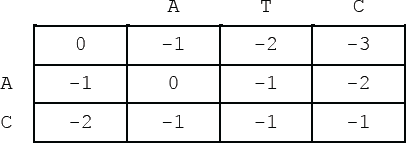
\includegraphics[width=0.4\textwidth]{fig03/dp_for_edit_distance.png}
\end{figure}
\vfill\null
\columnbreak

\vfill\null
\noindent $T = -1$ \\\\
\noindent $d = 1$

\end{multicols} 

%
% Metric space
%
\subsubsection*{Metric space}
The edit distance constitutes a metric space.
\begin{itemize}
\item $d_{xy} = 0$ for $x = y$ 
\item $d_{xy} > 0$ for $x \neq y$
\item $d_{xy} = d_{yx}$
\item $d_{xy} \leq d_{xz} + d_{zy}$ for any $z$ (the triangle inequality)
\end{itemize}

%
% Mutation and distance
%
\subsubsection*{Mutation and distance}
Mutations may occur several times on the same position.

\medskip 
\noindent
\textbf{Example of single mutations} \\

\noindent
$ACGT \rightarrow AGT \rightarrow ACT \rightarrow AGT \rightarrow AGCT$

\medskip 
\noindent
Four mutations have occurred, but the edit distance is 2.

%
% Mutation and distance
%
\subsubsection*{Distance per column}
It indicates the number of mutations per column (nucleotide/amino acid).

\bigskip 
$D = d / $(length of the longest sequence)

%
% Correction of distance
%
\subsubsection*{Correction of distance}
The distance can be adjusted. Below is a simple correction approach for protein sequences.

\bigskip 
$K=-\ln⁡(1-D-1/5 D^2 )$
\begin{figure}[H]
  \centering
      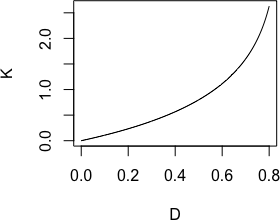
\includegraphics[width=0.3\textwidth]{fig03/adjust_distance.png}
      \caption{Correction of distance $D$}
\end{figure}

\medskip 
\noindent
\textbf{Example of distance correction} \\

$D = 0.5$

$K = -\ln⁡(1 - 0.5 - 1/5  \times 0.25 ) = -\ln(0.45) \approx 0.8⁡$

%\end{document}

